\subsection{Simulation}
We next demonstrate how the most efficient among different regularized estimators can reveal the structure of correlations.
We constructed four families of $50\times 50$ covariance matrices, each with structure that matched one of the four regularized estimators (Fig.~\ref{fig:1} Row 2, A--D and Methods).  We used these covariance matrices as the ground truth in multivariate Gaussian distributions with zero means and drew samples of various sizes. 
The sample correlation matrices from finite samples (\emph{e.g.}\ $n=500$ in Fig.~\ref{fig:1} Row 3) were contaminated with sampling noise and their underlying structures were difficult to discern.

The evaluation of any covariance matrix estimator, $C$, is performed with respect to a \emph{loss function} $\ell(C,\Sigma)$ to quantify its discrepancy from the truth, $\Sigma$.  The loss function is chosen to attain its minimum when $C=\Sigma$.
Here, in the role of the loss function we adopted the Kullback-Leibler divergence between multivariate normal distributions with equal means, scaled by $\frac 1 p$ to make its values comparable across different population sizes: 
\begin{equation}\label{eq:loss}
    \ell(C,\Sigma) = 
    \frac 1 p D_{KL}\left(\mathcal N_\Sigma\,\Vert\,\mathcal N_C\right) = 
    \frac 1 {2p} \left[\Tr(C^{-1}\Sigma) + \ln\det C - \ln\det\Sigma - p\right] 
\end{equation}
Therefore, $\ell(C,\Sigma)$ is expressed in nats/neuron per time bin.

We drew 30 independent samples with sample sizes $n=250$, 500, 1000, 2000, and 4000 from each model and computed the loss $\ell(C,\Sigma)$ for each of the five estimators.  
The hyperparameters of the regularized estimators were optimized by nested cross-validation using only the data in the sample.  
All the regularized estimators produced better estimates (lower loss) than the sample covariance matrix.  
However, estimators whose structure matched the true model outperformed the other estimators (Fig.~\ref{fig:1} Row 5).

Note that when the ground truth had zero correlations (Column A), $C_{\sf factor}$ performed equally well to $C_{\sf diag}$ because it correctly inferred zero factors and only estimated the individual variances. 
Similarly, when the number of latent units was zero (Column C), $C_{\sf sparse+latent}$ performed nearly equally well to $C_{\sf sparse}$ because it correctly inferred zero latent units.
With increasing sample sizes, all estimators converged to the truth (zero loss).  
However, the discriminability between their performances only increased with sample size (data not shown).

In more realistic conditions, when the ground truth is not accessible, the loss cannot be computed directly but may be estimated from data through \emph{validation}.
In a validation procedure, a validation sample covariance matrix $C_{\sf sample}^\prime$ is computed from a testing data set that is independent from the data used for computing $C$.
Then the \emph{validation loss} $\loss{C,C^\prime_{\sf sample}}$ measures the discrepancy of $C$ from $C^\prime_{\sf sample}$. 
Here, in the role of validation loss, we adopted the negative multivariate normal log likelihood of $C$ given $C^\prime_{\sf sample}$, also scaled by $\frac 1 p$ and omitting the constant term: 
\begin{equation}\label{eq:vloss}
    \loss{C,C^\prime_{\sf sample}} = \frac 1 {2p} \left[\Tr(C^{-1}C^\prime_{\sf sample})+\ln\det C \right]
\end{equation}

Since $\loss{\cdot,\cdot}$ is additive in its second argument and $C^\prime_{\sf sample}$ is an unbiased estimate of $\Sigma$, then, for given $C$ and $\Sigma$, the validation loss is an unbiased estimate of the true loss, up to a constant:
\begin{equation}
    \E{\loss{C,C_{\sf sample}^\prime}}=\loss{C,\E{C_{\sf sample}^\prime}}=\loss{C,\Sigma} = \ell(C,\Sigma) + \mbox{const}.
\end{equation}
Therefore, the validation procedure allows comparing the relative values of loss of different covariance estimators.

Indeed, the validation loss computed by 10-fold cross-validation (see Methods) accurately reproduces the relative values of the true loss and the rankings of the covariance estimators without access to the ground truth (Fig.~\ref{fig:1} Row 6). 

In the example above, the data were sampled from  multivariate normal random variables. In such models, partial correlations perfectly characterize the conditional dependencies between variables and the graphical models of partial correlations exactly correspond to the conditional dependencies in the data. 
To demonstrate that estimator rankings were robust to deviations from Gaussian models, we repeated the same cross-validated evaluation using pairwise Ising models to generate the data.

Ising models have been used to infer functional connectivity from neuronal spike trains \citep{Hertz:2011}. 
Conveniently, the Ising model has equivalent mathematical form to the Gaussian distribution,
\begin{equation}\label{eq:ising}
    x\sim \frac 1 {Z(J,h)} \exp\left(\frac 1 2 x^\T J x + h^\T x \right)
\end{equation}
but the Ising model is defined on the multivariate binary domain rather than the continuous domain. 
Both models are maximum-entropy models constrained to match the mean firing rates and the covariance matrix \citep{Jaynes:1957}.
The partition function $Z(J,h)$ normalizes the distribution on the models' respective domains. 
In the Gaussian model, the matrix $-J^{-1}$ is the covariance matrix; and the mean values are $\mu=J^{-1}h$.  
For the Ising model, $J$ is the matrix of pairwise interactions and $h$ is the vector of the cells' individual activity drives, although they do not have a simple relationship to the means and the covariance matrix. 
Both distributions have the same structure of pairwise conditional dependencies: zeros in the matrix $J$ indicate conditional independence between the corresponding pair of neurons. 

\begin{figure}
\begin{fullpage}
	\begin{center}
    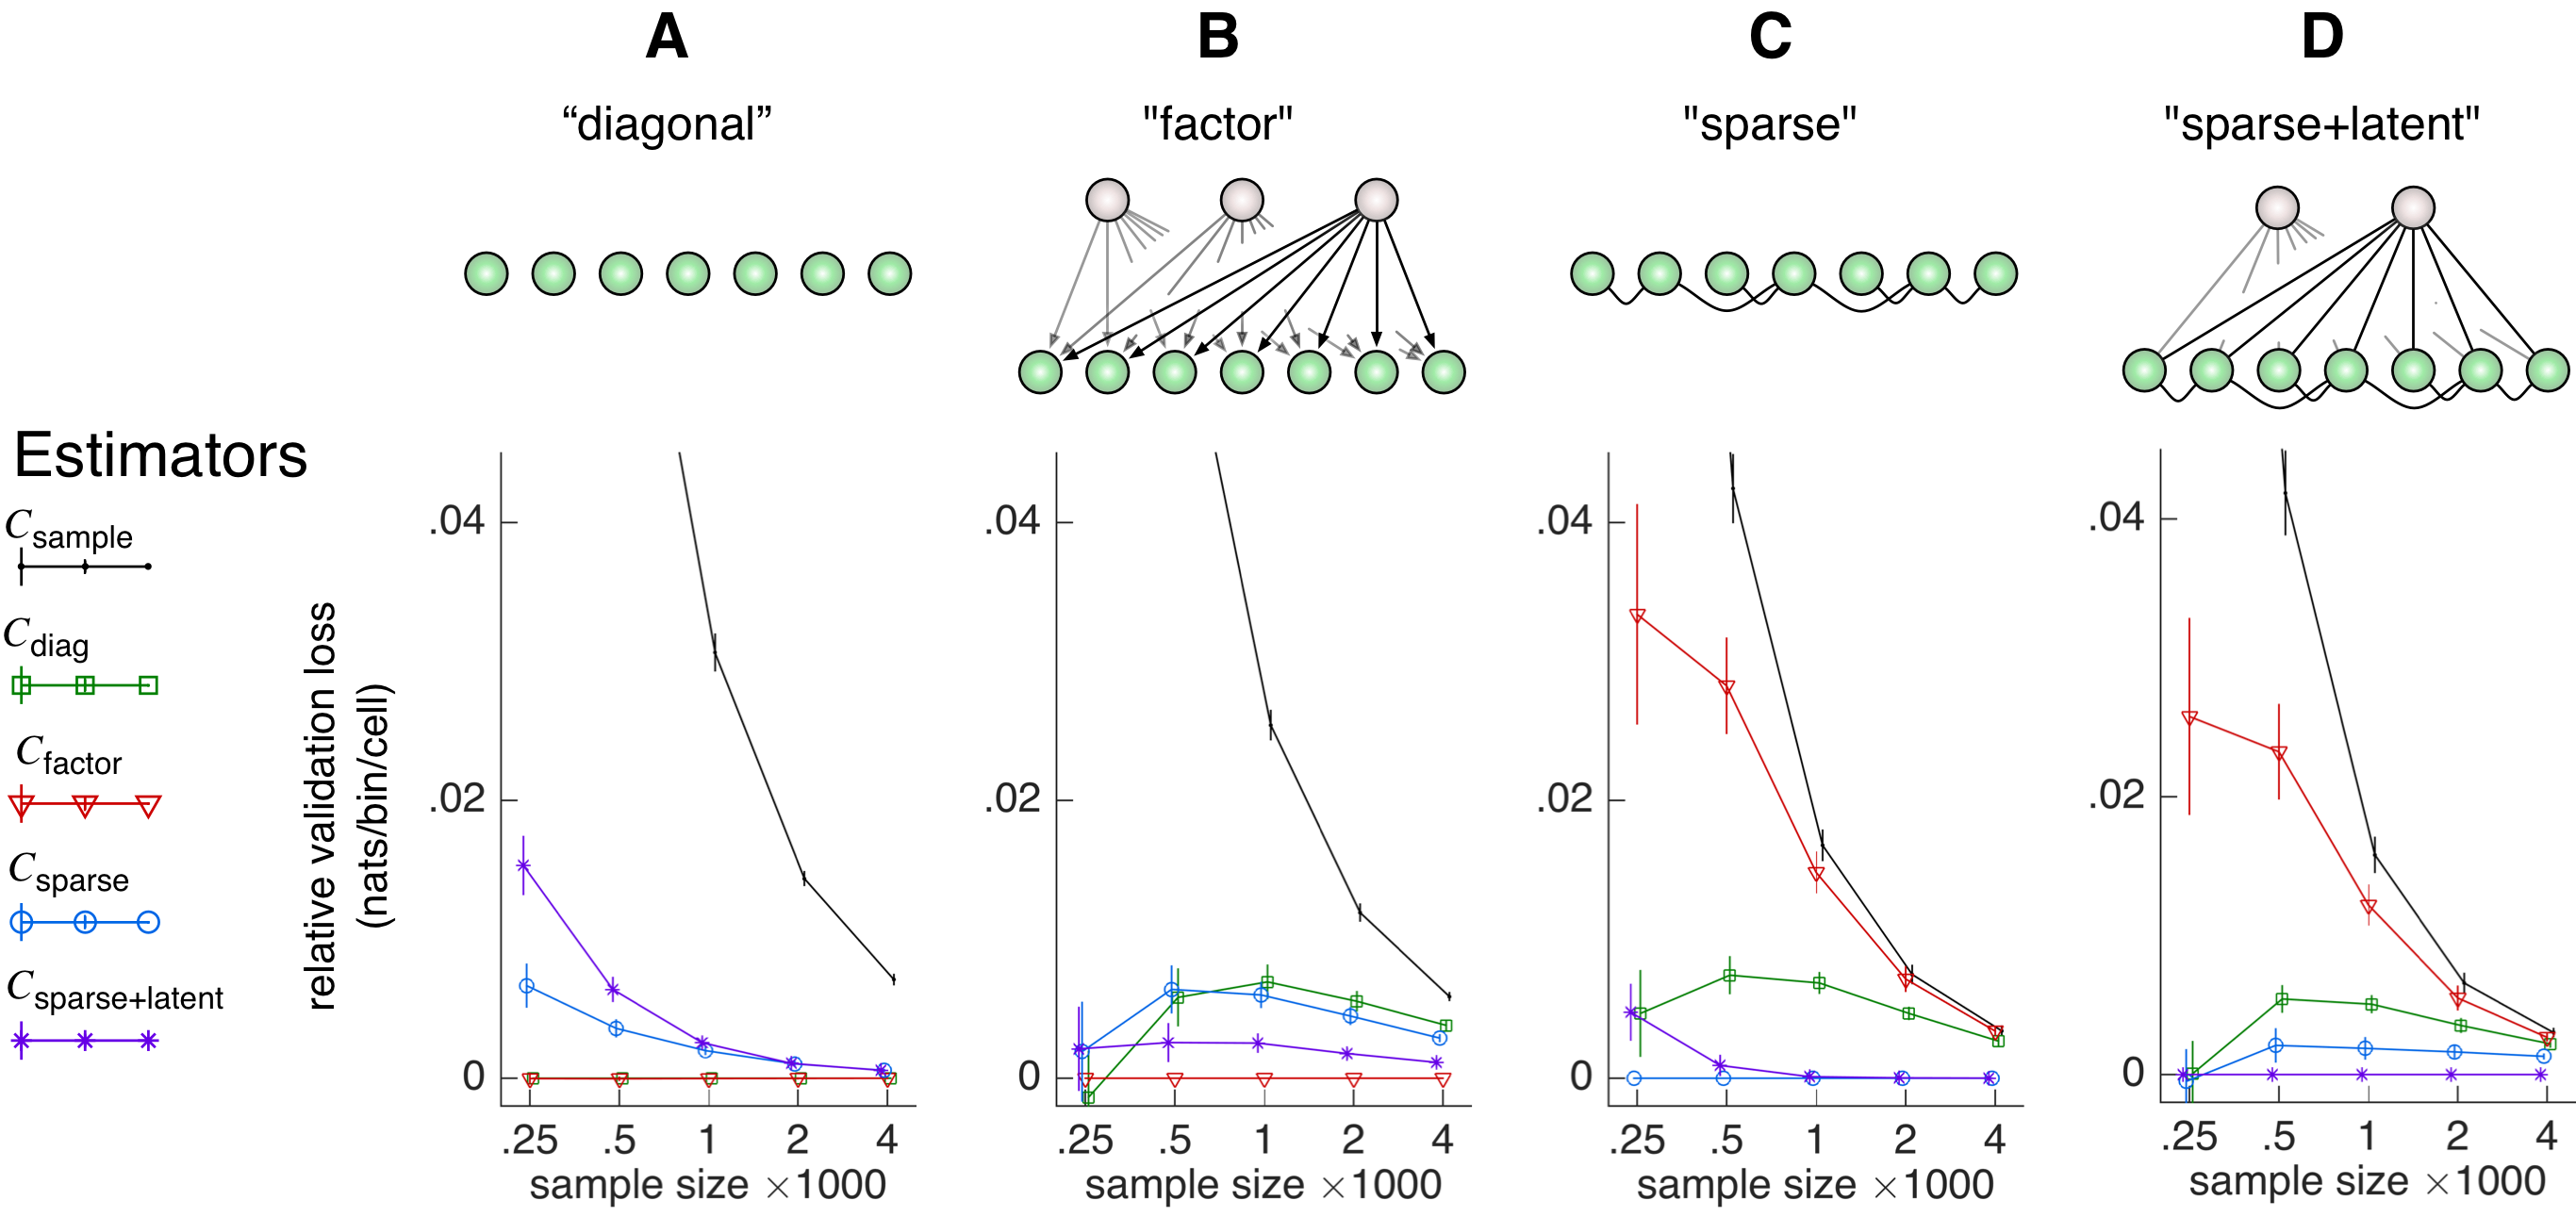
\includegraphics[width=\textwidth]{./figures/Figure2.png}
    \end{center}
\caption[Performance of covariance estimators on samples from Ising models]
{{\bf Performance of covariance estimators on samples from Ising models.}
{\bf A--D} Validation losses of covariance matrix estimators relative to the estimator whose structure matches the ground truth. The calculation is performed identically to Fig.~\ref{fig:1} Row 6 except Ising models are used as ground truth. 
}\label{fig:2}
\end{fullpage}
\end{figure}  %%%%%% FIGURE 2 from the paper

Indeed, despite their considerable departure from strictly linear conditional dependencies, Ising models yielded the same relationships between the performances of the covariance estimators as the Gaussian models in cross-validation (Fig.~\ref{fig:2}). Identical interaction matrices $J$  of the joint distributions over the observable and latent variables were used for both the Gaussian and the Ising models.

This simulation study demonstrated that cross-validated evaluation of regularized estimators of the covariance matrix of population activity can discriminate between structures of dependencies in the population. The identity of the most efficient covariance estimator for a particular neural circuit is therefore an empirical finding characterizing the nature of circuit  interactions.
